% Options for packages loaded elsewhere
\PassOptionsToPackage{unicode}{hyperref}
\PassOptionsToPackage{hyphens}{url}
%
\documentclass[
]{article}
\usepackage{lmodern}
\usepackage{amssymb,amsmath}
\usepackage{ifxetex,ifluatex}
\ifnum 0\ifxetex 1\fi\ifluatex 1\fi=0 % if pdftex
  \usepackage[T1]{fontenc}
  \usepackage[utf8]{inputenc}
  \usepackage{textcomp} % provide euro and other symbols
\else % if luatex or xetex
  \usepackage{unicode-math}
  \defaultfontfeatures{Scale=MatchLowercase}
  \defaultfontfeatures[\rmfamily]{Ligatures=TeX,Scale=1}
\fi
% Use upquote if available, for straight quotes in verbatim environments
\IfFileExists{upquote.sty}{\usepackage{upquote}}{}
\IfFileExists{microtype.sty}{% use microtype if available
  \usepackage[]{microtype}
  \UseMicrotypeSet[protrusion]{basicmath} % disable protrusion for tt fonts
}{}
\makeatletter
\@ifundefined{KOMAClassName}{% if non-KOMA class
  \IfFileExists{parskip.sty}{%
    \usepackage{parskip}
  }{% else
    \setlength{\parindent}{0pt}
    \setlength{\parskip}{6pt plus 2pt minus 1pt}}
}{% if KOMA class
  \KOMAoptions{parskip=half}}
\makeatother
\usepackage{xcolor}
\IfFileExists{xurl.sty}{\usepackage{xurl}}{} % add URL line breaks if available
\IfFileExists{bookmark.sty}{\usepackage{bookmark}}{\usepackage{hyperref}}
\hypersetup{
  pdftitle={Application to 2016 Election Data},
  hidelinks,
  pdfcreator={LaTeX via pandoc}}
\urlstyle{same} % disable monospaced font for URLs
\usepackage[margin=1in]{geometry}
\usepackage{color}
\usepackage{fancyvrb}
\newcommand{\VerbBar}{|}
\newcommand{\VERB}{\Verb[commandchars=\\\{\}]}
\DefineVerbatimEnvironment{Highlighting}{Verbatim}{commandchars=\\\{\}}
% Add ',fontsize=\small' for more characters per line
\usepackage{framed}
\definecolor{shadecolor}{RGB}{248,248,248}
\newenvironment{Shaded}{\begin{snugshade}}{\end{snugshade}}
\newcommand{\AlertTok}[1]{\textcolor[rgb]{0.94,0.16,0.16}{#1}}
\newcommand{\AnnotationTok}[1]{\textcolor[rgb]{0.56,0.35,0.01}{\textbf{\textit{#1}}}}
\newcommand{\AttributeTok}[1]{\textcolor[rgb]{0.77,0.63,0.00}{#1}}
\newcommand{\BaseNTok}[1]{\textcolor[rgb]{0.00,0.00,0.81}{#1}}
\newcommand{\BuiltInTok}[1]{#1}
\newcommand{\CharTok}[1]{\textcolor[rgb]{0.31,0.60,0.02}{#1}}
\newcommand{\CommentTok}[1]{\textcolor[rgb]{0.56,0.35,0.01}{\textit{#1}}}
\newcommand{\CommentVarTok}[1]{\textcolor[rgb]{0.56,0.35,0.01}{\textbf{\textit{#1}}}}
\newcommand{\ConstantTok}[1]{\textcolor[rgb]{0.00,0.00,0.00}{#1}}
\newcommand{\ControlFlowTok}[1]{\textcolor[rgb]{0.13,0.29,0.53}{\textbf{#1}}}
\newcommand{\DataTypeTok}[1]{\textcolor[rgb]{0.13,0.29,0.53}{#1}}
\newcommand{\DecValTok}[1]{\textcolor[rgb]{0.00,0.00,0.81}{#1}}
\newcommand{\DocumentationTok}[1]{\textcolor[rgb]{0.56,0.35,0.01}{\textbf{\textit{#1}}}}
\newcommand{\ErrorTok}[1]{\textcolor[rgb]{0.64,0.00,0.00}{\textbf{#1}}}
\newcommand{\ExtensionTok}[1]{#1}
\newcommand{\FloatTok}[1]{\textcolor[rgb]{0.00,0.00,0.81}{#1}}
\newcommand{\FunctionTok}[1]{\textcolor[rgb]{0.00,0.00,0.00}{#1}}
\newcommand{\ImportTok}[1]{#1}
\newcommand{\InformationTok}[1]{\textcolor[rgb]{0.56,0.35,0.01}{\textbf{\textit{#1}}}}
\newcommand{\KeywordTok}[1]{\textcolor[rgb]{0.13,0.29,0.53}{\textbf{#1}}}
\newcommand{\NormalTok}[1]{#1}
\newcommand{\OperatorTok}[1]{\textcolor[rgb]{0.81,0.36,0.00}{\textbf{#1}}}
\newcommand{\OtherTok}[1]{\textcolor[rgb]{0.56,0.35,0.01}{#1}}
\newcommand{\PreprocessorTok}[1]{\textcolor[rgb]{0.56,0.35,0.01}{\textit{#1}}}
\newcommand{\RegionMarkerTok}[1]{#1}
\newcommand{\SpecialCharTok}[1]{\textcolor[rgb]{0.00,0.00,0.00}{#1}}
\newcommand{\SpecialStringTok}[1]{\textcolor[rgb]{0.31,0.60,0.02}{#1}}
\newcommand{\StringTok}[1]{\textcolor[rgb]{0.31,0.60,0.02}{#1}}
\newcommand{\VariableTok}[1]{\textcolor[rgb]{0.00,0.00,0.00}{#1}}
\newcommand{\VerbatimStringTok}[1]{\textcolor[rgb]{0.31,0.60,0.02}{#1}}
\newcommand{\WarningTok}[1]{\textcolor[rgb]{0.56,0.35,0.01}{\textbf{\textit{#1}}}}
\usepackage{graphicx,grffile}
\makeatletter
\def\maxwidth{\ifdim\Gin@nat@width>\linewidth\linewidth\else\Gin@nat@width\fi}
\def\maxheight{\ifdim\Gin@nat@height>\textheight\textheight\else\Gin@nat@height\fi}
\makeatother
% Scale images if necessary, so that they will not overflow the page
% margins by default, and it is still possible to overwrite the defaults
% using explicit options in \includegraphics[width, height, ...]{}
\setkeys{Gin}{width=\maxwidth,height=\maxheight,keepaspectratio}
% Set default figure placement to htbp
\makeatletter
\def\fps@figure{htbp}
\makeatother
\setlength{\emergencystretch}{3em} % prevent overfull lines
\providecommand{\tightlist}{%
  \setlength{\itemsep}{0pt}\setlength{\parskip}{0pt}}
\setcounter{secnumdepth}{-\maxdimen} % remove section numbering
\usepackage{stackengine}
\usepackage{rotating}
\usepackage{booktabs}
\usepackage{longtable}
\usepackage{array}
\usepackage{multirow}
\usepackage{wrapfig}
\usepackage{float}
\usepackage{colortbl}
\usepackage{pdflscape}
\usepackage{tabu}
\usepackage{threeparttable}
\usepackage{threeparttablex}
\usepackage[normalem]{ulem}
\usepackage{makecell}
\usepackage{xcolor}

\title{Application to 2016 Election Data}
\author{}
\date{\vspace{-2.5em}}

\begin{document}
\maketitle

\begin{Shaded}
\begin{Highlighting}[]
\CommentTok{## Erin's path}
\NormalTok{path_data =}\StringTok{ "~/Dropbox/Documents/2019__2020/work/kpop/2016_reweighting_example/data/"}
\end{Highlighting}
\end{Shaded}

\begin{Shaded}
\begin{Highlighting}[]
\NormalTok{vote_contrast <-}\StringTok{ }\KeywordTok{quote}\NormalTok{((recode_vote_2016Democrat }\OperatorTok{-}\StringTok{ }\NormalTok{recode_vote_2016Republican) }\OperatorTok{/}
\StringTok{                           }\NormalTok{(recode_vote_2016Democrat }\OperatorTok{+}\StringTok{ }\NormalTok{recode_vote_2016Republican))}

\CommentTok{### Function for creating targets from auxiliary information and formula}
\NormalTok{create_targets <-}\StringTok{ }\ControlFlowTok{function}\NormalTok{ (target_design, target_formula) \{}
\NormalTok{    target_mf <-}\StringTok{ }\KeywordTok{model.frame}\NormalTok{(target_formula, }\KeywordTok{model.frame}\NormalTok{(target_design))}
\NormalTok{    target_mm <-}\StringTok{ }\KeywordTok{model.matrix}\NormalTok{(target_formula, target_mf)}
\NormalTok{    wts <-}\StringTok{ }\KeywordTok{weights}\NormalTok{(target_design)}
    \KeywordTok{colSums}\NormalTok{(target_mm }\OperatorTok{*}\StringTok{ }\NormalTok{wts) }\OperatorTok{/}\StringTok{ }\KeywordTok{sum}\NormalTok{(wts)}
\NormalTok{\}}
\end{Highlighting}
\end{Shaded}

\hypertarget{load-data}{%
\subsection{Load Data}\label{load-data}}

\begin{Shaded}
\begin{Highlighting}[]
\CommentTok{## SURVEY DATA (PEW)}
\CommentTok{### Load}
\CommentTok{###This needs to be loaded from dropbox/local not github bc it's too big}
\NormalTok{pew <-}\StringTok{ }\KeywordTok{readRDS}\NormalTok{(}\KeywordTok{paste0}\NormalTok{(path_data, }\StringTok{"pew.rds"}\NormalTok{))}

\CommentTok{## AUXILIARY INFORMATION (CCES)}
\CommentTok{### Load}
\CommentTok{#This needs to be loaded from dropbox/local not github bc it's too big}
\NormalTok{cces <-}\StringTok{ }\KeywordTok{readRDS}\NormalTok{(}\KeywordTok{paste0}\NormalTok{(path_data, }\StringTok{"cces.rds"}\NormalTok{))}
\CommentTok{### Drop invalid cases}
\NormalTok{cces <-}\StringTok{ }\NormalTok{cces }\OperatorTok
\StringTok{    }\KeywordTok{filter}\NormalTok{((CC16_}\DecValTok{401} \OperatorTok{==}\StringTok{ "I definitely voted in the General Election."}\NormalTok{) }\OperatorTok{&}
\StringTok{               }\OperatorTok{!}\KeywordTok{is.na}\NormalTok{(commonweight_vv_post))}

\CommentTok{## make recode_educ_white column}
\NormalTok{cces <-}\StringTok{ }\NormalTok{cces }\OperatorTok
\StringTok{  }\KeywordTok{mutate}\NormalTok{(}\DataTypeTok{recode_educ_white =} \KeywordTok{factor}\NormalTok{(}\KeywordTok{case_when}\NormalTok{(recode_race }\OperatorTok{==}\StringTok{ "White"} \OperatorTok{~}\StringTok{ }\KeywordTok{as.character}\NormalTok{(recode_educ),}
                               \OtherTok{TRUE} \OperatorTok{~}\StringTok{ "No Split"}\NormalTok{), }\DataTypeTok{levels =} \KeywordTok{c}\NormalTok{(}\KeywordTok{levels}\NormalTok{(cces}\OperatorTok{$}\NormalTok{recode_educ), }\StringTok{"No Split"}\NormalTok{)))}

\NormalTok{pew <-}\StringTok{ }\NormalTok{pew }\OperatorTok
\StringTok{  }\KeywordTok{mutate}\NormalTok{(}\DataTypeTok{recode_educ_white =} \KeywordTok{factor}\NormalTok{(}\KeywordTok{case_when}\NormalTok{(recode_race }\OperatorTok{==}\StringTok{ "White"} \OperatorTok{~}\StringTok{ }\KeywordTok{as.character}\NormalTok{(recode_educ),}
                               \OtherTok{TRUE} \OperatorTok{~}\StringTok{ "No Split"}\NormalTok{), }\DataTypeTok{levels =} \KeywordTok{c}\NormalTok{(}\KeywordTok{levels}\NormalTok{(pew}\OperatorTok{$}\NormalTok{recode_educ), }\StringTok{"No Split"}\NormalTok{)))}

\CommentTok{### Actual results}
\NormalTok{pres <-}\StringTok{ }\KeywordTok{readRDS}\NormalTok{(}\KeywordTok{paste0}\NormalTok{(path_data, }\StringTok{"election.rds"}\NormalTok{))}

\NormalTok{natl_margin <-}\StringTok{ }\NormalTok{pres }\OperatorTok
\StringTok{    }\KeywordTok{summarise}\NormalTok{(}\DataTypeTok{margin =}\NormalTok{ (}\KeywordTok{sum}\NormalTok{(demtotal) }\OperatorTok{-}\StringTok{ }\KeywordTok{sum}\NormalTok{(reptotal)) }\OperatorTok{/}
\StringTok{                  }\NormalTok{(}\KeywordTok{sum}\NormalTok{(demtotal) }\OperatorTok{+}\StringTok{ }\KeywordTok{sum}\NormalTok{(reptotal))) }\OperatorTok
\StringTok{    }\KeywordTok{as.numeric}\NormalTok{()}
\NormalTok{natl_margin}
\end{Highlighting}
\end{Shaded}

\begin{verbatim}
## [1] 0.02325013
\end{verbatim}

\begin{Shaded}
\begin{Highlighting}[]
\NormalTok{formula_rake_demos_noeduc <-}\StringTok{ }\ErrorTok{~}\NormalTok{recode_age_bucket }\OperatorTok{+}\StringTok{ }\NormalTok{recode_female }\OperatorTok{+}\StringTok{ }\NormalTok{recode_race }\OperatorTok{+}\StringTok{ }\NormalTok{recode_region }\OperatorTok{+}\StringTok{ }\NormalTok{recode_pid_3way}
\NormalTok{formula_rake_demos_weduc <-}\StringTok{ }\ErrorTok{~}\NormalTok{recode_age_bucket }\OperatorTok{+}\StringTok{ }\NormalTok{recode_female }\OperatorTok{+}\StringTok{ }\NormalTok{recode_race }\OperatorTok{+}\StringTok{ }\NormalTok{recode_region }\OperatorTok{+}\StringTok{ }
\StringTok{    }\NormalTok{recode_educ }\OperatorTok{+}\StringTok{ }\NormalTok{recode_pid_3way}
\NormalTok{formula_ps <-}\StringTok{ }\ErrorTok{~}\NormalTok{recode_age_3way }\OperatorTok{+}\StringTok{ }\NormalTok{recode_female }\OperatorTok{+}\StringTok{ }\NormalTok{recode_race }\OperatorTok{+}
\StringTok{    }\NormalTok{recode_region }\OperatorTok{+}\StringTok{ }\NormalTok{recode_educ_3way }\OperatorTok{+}\StringTok{ }\NormalTok{recode_pid_3way}
\CommentTok{#add interaction with pid}
\NormalTok{formula_retrospective <-}\StringTok{ }\ErrorTok{~}\NormalTok{recode_age_bucket}\OperatorTok{:}\NormalTok{recode_pid_3way }\OperatorTok{+}\StringTok{ }\NormalTok{recode_female}\OperatorTok{:}\NormalTok{recode_pid_3way}\OperatorTok{+}
\StringTok{    }\NormalTok{recode_race_educ_reg}\OperatorTok{:}\NormalTok{recode_pid_3way}
\end{Highlighting}
\end{Shaded}

\begin{Shaded}
\begin{Highlighting}[]
\CommentTok{## Find Missing Strata}
\CommentTok{## Make "strata" variable in CCES and Pew}
\NormalTok{cces <-}\StringTok{ }\KeywordTok{bind_cols}\NormalTok{(cces, cces }\OperatorTok\StringTok{ }
\StringTok{                    }\KeywordTok{unite}\NormalTok{(}\StringTok{"strata"}\NormalTok{, }\KeywordTok{all.vars}\NormalTok{(formula_ps), }\DataTypeTok{remove =} \OtherTok{FALSE}\NormalTok{) }\OperatorTok
\StringTok{                    }\KeywordTok{unite}\NormalTok{(}\StringTok{"strata_wage"}\NormalTok{, }\KeywordTok{c}\NormalTok{(}\KeywordTok{all.vars}\NormalTok{(formula_ps), }\StringTok{"recode_age"}\NormalTok{), }\DataTypeTok{remove =} \OtherTok{FALSE}\NormalTok{) }\OperatorTok
\StringTok{                    }\KeywordTok{select}\NormalTok{(strata, strata_wage))}

\NormalTok{pew <-}\StringTok{ }\KeywordTok{bind_cols}\NormalTok{(pew, pew }\OperatorTok\StringTok{ }
\StringTok{                   }\KeywordTok{unite}\NormalTok{(}\StringTok{"strata"}\NormalTok{, }\KeywordTok{all.vars}\NormalTok{(formula_ps), }\DataTypeTok{remove =} \OtherTok{FALSE}\NormalTok{) }\OperatorTok
\StringTok{                   }\KeywordTok{unite}\NormalTok{(}\StringTok{"strata_wage"}\NormalTok{, }\KeywordTok{c}\NormalTok{(}\KeywordTok{all.vars}\NormalTok{(formula_ps), }\StringTok{"recode_age"}\NormalTok{), }\DataTypeTok{remove =} \OtherTok{FALSE}\NormalTok{) }\OperatorTok
\StringTok{                   }\KeywordTok{select}\NormalTok{(strata, strata_wage))}


\NormalTok{missing_strata <-}\StringTok{ }\KeywordTok{unique}\NormalTok{(cces}\OperatorTok{$}\NormalTok{strata)[}\OperatorTok{!}\NormalTok{(}\KeywordTok{unique}\NormalTok{(cces}\OperatorTok{$}\NormalTok{strata) }\OperatorTok\StringTok{ }\KeywordTok{unique}\NormalTok{(pew}\OperatorTok{$}\NormalTok{strata))]}

\CommentTok{## recode missing age}
\NormalTok{pew}\OperatorTok{$}\NormalTok{recode_age[}\KeywordTok{is.na}\NormalTok{(pew}\OperatorTok{$}\NormalTok{recode_age)] <-}\StringTok{ }\KeywordTok{mean}\NormalTok{(pew}\OperatorTok{$}\NormalTok{recode_age, }\DataTypeTok{na.rm =} \OtherTok{TRUE}\NormalTok{)}
\NormalTok{cces}\OperatorTok{$}\NormalTok{recode_age[}\KeywordTok{is.na}\NormalTok{(cces}\OperatorTok{$}\NormalTok{recode_age)] <-}\StringTok{ }\KeywordTok{mean}\NormalTok{(cces}\OperatorTok{$}\NormalTok{recode_age, }\DataTypeTok{na.rm =} \OtherTok{TRUE}\NormalTok{)}

\CommentTok{### Make survey designs}

\CommentTok{## For Pew, since there are no design weights, assume SRS}
\NormalTok{pew_srs <-}\StringTok{ }\KeywordTok{svydesign}\NormalTok{(}\DataTypeTok{ids =} \OperatorTok{~}\DecValTok{1}\NormalTok{, }\DataTypeTok{data =}\NormalTok{ pew)}
\end{Highlighting}
\end{Shaded}

\begin{verbatim}
## Warning in svydesign.default(ids = ~1, data = pew): No weights or probabilities
## supplied, assuming equal probability
\end{verbatim}

\begin{Shaded}
\begin{Highlighting}[]
\NormalTok{cces_awt <-}\StringTok{ }\KeywordTok{svydesign}\NormalTok{(}\DataTypeTok{ids =} \OperatorTok{~}\DecValTok{1}\NormalTok{, }\DataTypeTok{weights =} \OperatorTok{~}\NormalTok{commonweight_vv_post, }\DataTypeTok{data =}\NormalTok{ cces)}
\end{Highlighting}
\end{Shaded}

\begin{Shaded}
\begin{Highlighting}[]
\CommentTok{### Population targets}
\NormalTok{targets_rake_demos_noeduc <-}\StringTok{ }\KeywordTok{create_targets}\NormalTok{(cces_awt, formula_rake_demos_noeduc)}
\NormalTok{targets_rake_demos_weduc <-}\StringTok{ }\KeywordTok{create_targets}\NormalTok{(cces_awt, formula_rake_demos_weduc)}
\NormalTok{targets_retrospective <-}\StringTok{ }\KeywordTok{create_targets}\NormalTok{(cces_awt, formula_retrospective)}
\end{Highlighting}
\end{Shaded}

\begin{Shaded}
\begin{Highlighting}[]
\CommentTok{## Raking on demographics, excluding education}
\NormalTok{rake_demos_noeduc <-}\StringTok{ }\KeywordTok{calibrate}\NormalTok{(}\DataTypeTok{design =}\NormalTok{ pew_srs,}
                       \DataTypeTok{formula =}\NormalTok{ formula_rake_demos_noeduc,}
                       \DataTypeTok{population =}\NormalTok{ targets_rake_demos_noeduc,}
                       \DataTypeTok{calfun =} \StringTok{"raking"}\NormalTok{)}

\NormalTok{rake_demos_noeduc <-}\StringTok{ }\KeywordTok{svydesign}\NormalTok{(}\OperatorTok{~}\DecValTok{1}\NormalTok{, }\DataTypeTok{data =}\NormalTok{ pew, }\DataTypeTok{weights =} \KeywordTok{weights}\NormalTok{(rake_demos_noeduc))}

\CommentTok{## Raking on demographics, including education}
\NormalTok{rake_demos_weduc <-}\StringTok{ }\KeywordTok{calibrate}\NormalTok{(}\DataTypeTok{design =}\NormalTok{ pew_srs,}
                              \DataTypeTok{formula =}\NormalTok{ formula_rake_demos_weduc,}
                              \DataTypeTok{population =}\NormalTok{ targets_rake_demos_weduc,}
                              \DataTypeTok{calfun =} \StringTok{"raking"}\NormalTok{)}

\NormalTok{rake_demos_weduc <-}\StringTok{ }\KeywordTok{svydesign}\NormalTok{(}\OperatorTok{~}\DecValTok{1}\NormalTok{, }\DataTypeTok{data =}\NormalTok{ pew, }\DataTypeTok{weights =} \KeywordTok{weights}\NormalTok{(rake_demos_weduc))}

\CommentTok{## Post-stratification}
\NormalTok{targets_ps <-}\StringTok{ }\KeywordTok{svytable}\NormalTok{(}\DataTypeTok{formula =} \OperatorTok{~}\NormalTok{strata, }\DataTypeTok{design =} \KeywordTok{subset}\NormalTok{(cces_awt, }\OperatorTok{!}\NormalTok{(strata }\OperatorTok\StringTok{ }\NormalTok{missing_strata)))}
\NormalTok{post_stratification <-}\StringTok{ }\KeywordTok{postStratify}\NormalTok{(}\DataTypeTok{design =}\NormalTok{ pew_srs,}
                         \DataTypeTok{strata =} \OperatorTok{~}\NormalTok{strata,}
                         \DataTypeTok{population =}\NormalTok{ targets_ps)}

\NormalTok{post_stratification <-}\StringTok{ }\KeywordTok{svydesign}\NormalTok{(}\OperatorTok{~}\DecValTok{1}\NormalTok{, }\DataTypeTok{data =}\NormalTok{ pew, }\DataTypeTok{weights =} \KeywordTok{weights}\NormalTok{(post_stratification))}

\CommentTok{## Retrospective weighting scheme}
\NormalTok{rake_retrospective <-}\StringTok{ }\KeywordTok{calibrate}\NormalTok{(}\DataTypeTok{design =}\NormalTok{ pew_srs,}
                              \DataTypeTok{formula =}\NormalTok{ formula_retrospective,}
                              \DataTypeTok{population =}\NormalTok{ targets_retrospective,}
                              \DataTypeTok{calfun =} \StringTok{"raking"}\NormalTok{,}
                              \DataTypeTok{force =} \OtherTok{TRUE}\NormalTok{)}
\end{Highlighting}
\end{Shaded}

\begin{verbatim}
## Warning in grake(mm, ww, calfun, bounds = bounds, population = population, :
## Failed to converge: eps=0.00688873036014645 in 51 iterations
\end{verbatim}

\begin{Shaded}
\begin{Highlighting}[]
\NormalTok{rake_retrospective <-}\StringTok{ }\KeywordTok{svydesign}\NormalTok{(}\OperatorTok{~}\DecValTok{1}\NormalTok{, }\DataTypeTok{data =}\NormalTok{ pew, }\DataTypeTok{weights =} \KeywordTok{weights}\NormalTok{(rake_retrospective))}
\end{Highlighting}
\end{Shaded}

\begin{Shaded}
\begin{Highlighting}[]
\CommentTok{#############################################}
\CommentTok{##### PUT FINAL KPOP CODE HERE}
\CommentTok{#############################################}

\KeywordTok{load}\NormalTok{(}\StringTok{"./cleaned data/Full SVD/weights_wPid_full.Rdata"}\NormalTok{)}

\NormalTok{kpop <-}\StringTok{ }\KeywordTok{svydesign}\NormalTok{(}\OperatorTok{~}\DecValTok{1}\NormalTok{, }\DataTypeTok{data =}\NormalTok{ pew, }\DataTypeTok{weights =}\NormalTok{ wts_wPid[, }\StringTok{"wtkbal_b.5x"}\NormalTok{])}
\NormalTok{kpop_mf <-}\StringTok{ }\KeywordTok{svydesign}\NormalTok{(}\OperatorTok{~}\DecValTok{1}\NormalTok{, }\DataTypeTok{data =}\NormalTok{ pew, }\DataTypeTok{weights =}\NormalTok{ wts_wPid[, }\StringTok{"wtkbal_mf_b2x"}\NormalTok{])}
\end{Highlighting}
\end{Shaded}

\begin{Shaded}
\begin{Highlighting}[]
\NormalTok{margin_summary <-}\StringTok{ }\KeywordTok{round}\NormalTok{(}\KeywordTok{cbind}\NormalTok{(}\DataTypeTok{cces =} \KeywordTok{svymean}\NormalTok{(formula_rake_demos_weduc, cces_awt),}
                              \DataTypeTok{unweighted =} \KeywordTok{svymean}\NormalTok{(formula_rake_demos_weduc, pew_srs),}
            \DataTypeTok{rake_demos_noeduc =} \KeywordTok{svymean}\NormalTok{(formula_rake_demos_weduc, rake_demos_noeduc),}
            \DataTypeTok{rake_demos_weduc =} \KeywordTok{svymean}\NormalTok{(formula_rake_demos_weduc, rake_demos_weduc),}
            \DataTypeTok{post_stratification =} \KeywordTok{svymean}\NormalTok{(formula_rake_demos_weduc, post_stratification),}
            \DataTypeTok{rake_retrospective =} \KeywordTok{svymean}\NormalTok{(formula_rake_demos_weduc, rake_retrospective),}
            \DataTypeTok{kpop =} \KeywordTok{svymean}\NormalTok{(formula_rake_demos_weduc, kpop),}
            \DataTypeTok{kpop_mf =} \KeywordTok{svymean}\NormalTok{(formula_rake_demos_weduc, kpop_mf)) }\OperatorTok{*}\StringTok{ }\DecValTok{100}\NormalTok{, }\DecValTok{1}\NormalTok{) }\OperatorTok
\StringTok{  }\KeywordTok{data.frame}\NormalTok{() }\OperatorTok
\StringTok{  }\KeywordTok{rownames_to_column}\NormalTok{() }\OperatorTok
\StringTok{  }\KeywordTok{mutate}\NormalTok{(}\DataTypeTok{variable =} \KeywordTok{case_when}\NormalTok{(}\KeywordTok{str_detect}\NormalTok{(rowname, }\StringTok{"age"}\NormalTok{) }\OperatorTok{~}\StringTok{ "4-way Age Bucket"}\NormalTok{,}
                             \KeywordTok{str_detect}\NormalTok{(rowname, }\StringTok{"female"}\NormalTok{) }\OperatorTok{~}\StringTok{ "Gender"}\NormalTok{,}
                             \KeywordTok{str_detect}\NormalTok{(rowname, }\StringTok{"race"}\NormalTok{) }\OperatorTok{~}\StringTok{ "Race/Ethnicity"}\NormalTok{,}
                             \KeywordTok{str_detect}\NormalTok{(rowname, }\StringTok{"region"}\NormalTok{) }\OperatorTok{~}\StringTok{ "Region"}\NormalTok{,}
                             \KeywordTok{str_detect}\NormalTok{(rowname, }\StringTok{"educ"}\NormalTok{) }\OperatorTok{~}\StringTok{ "Education Level"}\NormalTok{,}
                             \KeywordTok{str_detect}\NormalTok{(rowname, }\StringTok{"pid"}\NormalTok{) }\OperatorTok{~}\StringTok{ "Party Identification"}\NormalTok{,}
                             \OtherTok{TRUE} \OperatorTok{~}\StringTok{ "Empty"}\NormalTok{),}
         \DataTypeTok{level =} \KeywordTok{gsub}\NormalTok{(}\StringTok{"recode_|age_bucket|female|race|region|educ|pid_3way"}\NormalTok{, }\StringTok{""}\NormalTok{, rowname)) }\OperatorTok
\StringTok{  }\KeywordTok{select}\NormalTok{(level, }\KeywordTok{everything}\NormalTok{(), }\OperatorTok{-}\NormalTok{rowname, }\OperatorTok{-}\NormalTok{variable)}
\end{Highlighting}
\end{Shaded}

\begin{table}

\caption{\label{tab:margins_table}Marginal distribution of important demographics under different weighting models.}
\centering
\begin{tabular}[t]{>{\raggedright\arraybackslash}p{1.35in}>{\raggedleft\arraybackslash}p{0.5in}>{\raggedleft\arraybackslash}p{0.5in}>{\raggedleft\arraybackslash}p{0.5in}>{\raggedleft\arraybackslash}p{0.5in}>{\raggedleft\arraybackslash}p{0.5in}>{\raggedleft\arraybackslash}p{0.5in}>{\raggedleft\arraybackslash}p{0.5in}>{\raggedleft\arraybackslash}p{0.5in}}
\toprule
 & \belowbaseline[0ex]{\rotatebox{90}{\parbox{1.1in}{\raggedright{Target (CCES)}}}} & \belowbaseline[0ex]{\rotatebox{90}{\parbox{1.1in}{\raggedright{Unweighted Pew}}}} & \belowbaseline[0ex]{\rotatebox{90}{\parbox{1.1in}{\raggedright{Raking \\Demographics No Education }}}} & \belowbaseline[0ex]{\rotatebox{90}{\parbox{1.1in}{\raggedright{Raking \\Demographics with Education }}}} & \belowbaseline[0ex]{\rotatebox{90}{\parbox{1.1in}{\raggedright{Post-Stratification}}}} & \belowbaseline[0ex]{\rotatebox{90}{\parbox{1.1in}{\raggedright{Raking Retrospective}}}} & \belowbaseline[0ex]{\rotatebox{90}{\parbox{1.1in}{\raggedright{Kpop}}}} & \belowbaseline[0ex]{\rotatebox{90}{\parbox{1.1in}{\raggedright{Kpop Mean First}}}}\\
\midrule
\addlinespace[0.5em]
\multicolumn{9}{l}{\textbf{4-way Age Bucket}}\\
\hspace{1em}18 to 35 & 34.8 & 43.7 & 34.8 & 34.8 & 35.4 & 34.8 & 34.4 & 34.8\\
\hspace{1em}36 to 50 & 22.6 & 32.6 & 22.6 & 22.6 & 26.7 & 22.6 & 23.6 & 22.6\\
\hspace{1em}51 to 64 & 28.9 & 21.0 & 28.9 & 28.9 & 29.7 & 28.9 & 29.5 & 28.9\\
\hspace{1em}65+ & 13.7 & 2.7 & 13.7 & 13.7 & 8.3 & 13.7 & 12.5 & 13.7\\
\addlinespace[0.5em]
\multicolumn{9}{l}{\textbf{Gender}}\\
\hspace{1em}Female & 50.8 & 47.3 & 50.8 & 50.8 & 50.8 & 50.8 & 50.8 & 50.8\\
\hspace{1em}Male & 49.2 & 52.7 & 49.2 & 49.2 & 49.2 & 49.2 & 49.2 & 49.2\\
\addlinespace[0.5em]
\multicolumn{9}{l}{\textbf{Race/Ethnicity}}\\
\hspace{1em}Black & 11.8 & 8.9 & 11.8 & 11.8 & 11.5 & 13.4 & 11.7 & 11.8\\
\hspace{1em}Hispanic & 6.5 & 7.6 & 6.5 & 6.5 & 6.2 & 6.5 & 5.9 & 6.5\\
\hspace{1em}Other & 6.8 & 7.1 & 6.8 & 6.8 & 6.5 & 6.8 & 6.2 & 6.8\\
\hspace{1em}White & 74.9 & 76.4 & 74.9 & 74.9 & 75.8 & 73.2 & 76.3 & 74.9\\
\addlinespace[0.5em]
\multicolumn{9}{l}{\textbf{Region}}\\
\hspace{1em}Midwest & 23.4 & 22.3 & 23.4 & 23.4 & 23.2 & 24.7 & 23.6 & 23.4\\
\hspace{1em}Northeast & 19.7 & 18.2 & 19.7 & 19.7 & 19.3 & 19.7 & 19.5 & 19.7\\
\hspace{1em}South & 35.5 & 37.9 & 35.5 & 35.5 & 36.9 & 34.8 & 36.0 & 35.5\\
\hspace{1em}West & 21.4 & 21.6 & 21.4 & 21.4 & 20.6 & 20.8 & 20.8 & 21.4\\
\addlinespace[0.5em]
\multicolumn{9}{l}{\textbf{Education Level}}\\
\hspace{1em}No HS & 6.8 & 1.8 & 1.8 & 6.8 & 2.4 & 3.6 & 1.9 & 6.8\\
\hspace{1em}High school & 30.6 & 19.7 & 21.5 & 30.6 & 28.8 & 29.4 & 31.2 & 30.6\\
\hspace{1em}Some college & 23.0 & 16.7 & 17.7 & 23.0 & 24.5 & 23.0 & 24.4 & 23.0\\
\hspace{1em}2-year & 10.6 & 11.3 & 10.6 & 10.6 & 9.5 & 11.7 & 10.9 & 10.6\\
\hspace{1em}4-year & 18.7 & 28.6 & 26.2 & 18.7 & 22.2 & 20.2 & 20.3 & 18.7\\
\hspace{1em}Post-grad & 10.4 & 21.9 & 22.3 & 10.4 & 12.6 & 12.2 & 11.3 & 10.4\\
\addlinespace[0.5em]
\multicolumn{9}{l}{\textbf{Party Identification}}\\
\hspace{1em}Dem & 38.1 & 34.4 & 38.1 & 38.1 & 38.5 & 38.1 & 37.6 & 38.1\\
\hspace{1em}Ind & 32.5 & 35.2 & 32.5 & 32.5 & 32.5 & 32.5 & 32.8 & 32.5\\
\hspace{1em}Rep & 29.5 & 30.4 & 29.5 & 29.5 & 29.0 & 29.5 & 29.5 & 29.5\\
\bottomrule
\end{tabular}
\end{table}

\begin{Shaded}
\begin{Highlighting}[]
\NormalTok{margin_summary_educ <-}\StringTok{ }\KeywordTok{round}\NormalTok{(}\KeywordTok{cbind}\NormalTok{(}\DataTypeTok{cces =} \KeywordTok{svymean}\NormalTok{(}\OperatorTok{~}\NormalTok{recode_educ_white, cces_awt),}
                              \DataTypeTok{unweighted =} \KeywordTok{svymean}\NormalTok{(}\OperatorTok{~}\NormalTok{recode_educ_white, pew_srs),}
            \DataTypeTok{rake_demos_noeduc =} \KeywordTok{svymean}\NormalTok{(}\OperatorTok{~}\NormalTok{recode_educ_white, rake_demos_noeduc),}
            \DataTypeTok{rake_demos_weduc =} \KeywordTok{svymean}\NormalTok{(}\OperatorTok{~}\NormalTok{recode_educ_white, rake_demos_weduc),}
            \DataTypeTok{post_stratification =} \KeywordTok{svymean}\NormalTok{(}\OperatorTok{~}\NormalTok{recode_educ_white, post_stratification),}
            \DataTypeTok{rake_retrospective =} \KeywordTok{svymean}\NormalTok{(}\OperatorTok{~}\NormalTok{recode_educ_white, rake_retrospective),}
            \DataTypeTok{kpop =} \KeywordTok{svymean}\NormalTok{(}\OperatorTok{~}\NormalTok{recode_educ_white, kpop),}
            \DataTypeTok{kpop_mf =} \KeywordTok{svymean}\NormalTok{(}\OperatorTok{~}\NormalTok{recode_educ_white, kpop_mf)) }\OperatorTok{*}\StringTok{ }\DecValTok{100}\NormalTok{, }\DecValTok{1}\NormalTok{) }\OperatorTok
\StringTok{  }\KeywordTok{data.frame}\NormalTok{() }\OperatorTok
\StringTok{  }\KeywordTok{rownames_to_column}\NormalTok{() }\OperatorTok
\StringTok{  }\KeywordTok{mutate}\NormalTok{(}\DataTypeTok{variable =} \KeywordTok{case_when}\NormalTok{(}\KeywordTok{str_detect}\NormalTok{(rowname, }\StringTok{"age"}\NormalTok{) }\OperatorTok{~}\StringTok{ "4-way Age Bucket"}\NormalTok{,}
                             \KeywordTok{str_detect}\NormalTok{(rowname, }\StringTok{"female"}\NormalTok{) }\OperatorTok{~}\StringTok{ "Gender"}\NormalTok{,}
                             \KeywordTok{str_detect}\NormalTok{(rowname, }\StringTok{"race"}\NormalTok{) }\OperatorTok{~}\StringTok{ "Race/Ethnicity"}\NormalTok{,}
                             \KeywordTok{str_detect}\NormalTok{(rowname, }\StringTok{"region"}\NormalTok{) }\OperatorTok{~}\StringTok{ "Region"}\NormalTok{,}
                             \KeywordTok{str_detect}\NormalTok{(rowname, }\StringTok{"educ"}\NormalTok{) }\OperatorTok{~}\StringTok{ "Education Level"}\NormalTok{,}
                             \KeywordTok{str_detect}\NormalTok{(rowname, }\StringTok{"pid"}\NormalTok{) }\OperatorTok{~}\StringTok{ "Party Identification"}\NormalTok{,}
                             \OtherTok{TRUE} \OperatorTok{~}\StringTok{ "Empty"}\NormalTok{),}
         \DataTypeTok{level =} \KeywordTok{gsub}\NormalTok{(}\StringTok{"recode_|age_bucket|female|race|region|educ|pid_3way|educ_3way|_white"}\NormalTok{, }\StringTok{""}\NormalTok{, rowname)) }\OperatorTok
\StringTok{  }\KeywordTok{select}\NormalTok{(level, }\KeywordTok{everything}\NormalTok{(), }\OperatorTok{-}\NormalTok{rowname, }\OperatorTok{-}\NormalTok{variable)}
\end{Highlighting}
\end{Shaded}

\begin{table}

\caption{\label{tab:margins_table_educ}Marginal distribution of education level for white voters under different weighting models.}
\centering
\begin{tabular}[t]{>{\raggedright\arraybackslash}p{1.35in}>{\raggedleft\arraybackslash}p{0.5in}>{\raggedleft\arraybackslash}p{0.5in}>{\raggedleft\arraybackslash}p{0.5in}>{\raggedleft\arraybackslash}p{0.5in}>{\raggedleft\arraybackslash}p{0.5in}>{\raggedleft\arraybackslash}p{0.5in}>{\raggedleft\arraybackslash}p{0.5in}>{\raggedleft\arraybackslash}p{0.5in}}
\toprule
 & \belowbaseline[0ex]{\rotatebox{90}{\parbox{1.1in}{\raggedright{Target (CCES)}}}} & \belowbaseline[0ex]{\rotatebox{90}{\parbox{1.1in}{\raggedright{Unweighted Pew}}}} & \belowbaseline[0ex]{\rotatebox{90}{\parbox{1.1in}{\raggedright{Raking \\Demographics No Education }}}} & \belowbaseline[0ex]{\rotatebox{90}{\parbox{1.1in}{\raggedright{Raking \\Demographics with Education }}}} & \belowbaseline[0ex]{\rotatebox{90}{\parbox{1.1in}{\raggedright{Post-Stratification}}}} & \belowbaseline[0ex]{\rotatebox{90}{\parbox{1.1in}{\raggedright{Raking Retrospective}}}} & \belowbaseline[0ex]{\rotatebox{90}{\parbox{1.1in}{\raggedright{Kpop}}}} & \belowbaseline[0ex]{\rotatebox{90}{\parbox{1.1in}{\raggedright{Kpop Mean First}}}}\\
\midrule
\addlinespace[0.5em]
\multicolumn{9}{l}{\textbf{Education Level for White Voters}}\\
\hspace{1em}No HS & 4.6 & 1.1 & 1.1 & 4.5 & 1.8 & 3.0 & 1.2 & 4.8\\
\hspace{1em}High school & 22.6 & 14.6 & 15.5 & 22.9 & 23.1 & 22.6 & 23.6 & 21.9\\
\hspace{1em}Some college & 16.9 & 11.5 & 12.1 & 16.3 & 19.5 & 16.9 & 18.3 & 17.7\\
\hspace{1em}2-year & 7.8 & 8.3 & 7.0 & 7.3 & 6.1 & 7.8 & 7.7 & 7.2\\
\hspace{1em}4-year & 14.8 & 23.0 & 20.7 & 15.2 & 17.1 & 14.8 & 16.3 & 14.8\\
\hspace{1em}Post-grad & 8.3 & 18.0 & 18.5 & 8.8 & 8.2 & 8.3 & 9.1 & 8.4\\
\bottomrule
\end{tabular}
\end{table}

\begin{Shaded}
\begin{Highlighting}[]
\NormalTok{target_margin <-}\StringTok{ }\KeywordTok{svycontrast}\NormalTok{(}\KeywordTok{svymean}\NormalTok{(}\OperatorTok{~}\NormalTok{recode_vote_}\DecValTok{2016}\NormalTok{, cces_awt, }\DataTypeTok{na.rm =} \OtherTok{TRUE}\NormalTok{),}
\NormalTok{                       vote_contrast)[}\DecValTok{1}\NormalTok{]}

\NormalTok{comp_df <-}\StringTok{ }\KeywordTok{data.frame}\NormalTok{(}
    \DataTypeTok{cces =} \KeywordTok{svycontrast}\NormalTok{(}\KeywordTok{svymean}\NormalTok{(}\OperatorTok{~}\NormalTok{recode_vote_}\DecValTok{2016}\NormalTok{, cces_awt, }\DataTypeTok{na.rm =} \OtherTok{TRUE}\NormalTok{),}
\NormalTok{                       vote_contrast),}
    \DataTypeTok{unweighted =} \KeywordTok{svycontrast}\NormalTok{(}\KeywordTok{svymean}\NormalTok{(}\OperatorTok{~}\NormalTok{recode_vote_}\DecValTok{2016}\NormalTok{, pew_srs, }\DataTypeTok{na.rm =} \OtherTok{TRUE}\NormalTok{),}
\NormalTok{                        vote_contrast),}
    \DataTypeTok{rake_demos_noeduc =} \KeywordTok{svycontrast}\NormalTok{(}\KeywordTok{svymean}\NormalTok{(}\OperatorTok{~}\NormalTok{recode_vote_}\DecValTok{2016}\NormalTok{, rake_demos_noeduc, }\DataTypeTok{na.rm =} \OtherTok{TRUE}\NormalTok{),}
\NormalTok{                        vote_contrast),}
    \DataTypeTok{rake_demos_weduc =} \KeywordTok{svycontrast}\NormalTok{(}\KeywordTok{svymean}\NormalTok{(}\OperatorTok{~}\NormalTok{recode_vote_}\DecValTok{2016}\NormalTok{, rake_demos_weduc, }\DataTypeTok{na.rm =} \OtherTok{TRUE}\NormalTok{),}
\NormalTok{                        vote_contrast),}
    \DataTypeTok{post_stratification =} \KeywordTok{svycontrast}\NormalTok{(}\KeywordTok{svymean}\NormalTok{(}\OperatorTok{~}\NormalTok{recode_vote_}\DecValTok{2016}\NormalTok{, post_stratification, }\DataTypeTok{na.rm =} \OtherTok{TRUE}\NormalTok{),}
\NormalTok{                        vote_contrast),}
    \DataTypeTok{rake_retrospective =} \KeywordTok{svycontrast}\NormalTok{(}\KeywordTok{svymean}\NormalTok{(}\OperatorTok{~}\NormalTok{recode_vote_}\DecValTok{2016}\NormalTok{, rake_retrospective, }\DataTypeTok{na.rm =} \OtherTok{TRUE}\NormalTok{),}
\NormalTok{                        vote_contrast),}
    \DataTypeTok{kpop =} \KeywordTok{svycontrast}\NormalTok{(}\KeywordTok{svymean}\NormalTok{(}\OperatorTok{~}\NormalTok{recode_vote_}\DecValTok{2016}\NormalTok{, kpop, }\DataTypeTok{na.rm =} \OtherTok{TRUE}\NormalTok{),}
\NormalTok{                        vote_contrast),}
    \DataTypeTok{kpop_mf =} \KeywordTok{svycontrast}\NormalTok{(}\KeywordTok{svymean}\NormalTok{(}\OperatorTok{~}\NormalTok{recode_vote_}\DecValTok{2016}\NormalTok{, kpop_mf, }\DataTypeTok{na.rm =} \OtherTok{TRUE}\NormalTok{),}
\NormalTok{                        vote_contrast)) }\OperatorTok
\StringTok{    }\KeywordTok{pivot_longer}\NormalTok{(}\DataTypeTok{cols =} \KeywordTok{everything}\NormalTok{(),}
                 \DataTypeTok{names_to =} \KeywordTok{c}\NormalTok{(}\StringTok{"source"}\NormalTok{, }\StringTok{".value"}\NormalTok{), }
                 \DataTypeTok{names_pattern =} \StringTok{"(.*)}\CharTok{\textbackslash{}\textbackslash{}}\StringTok{.(.*)"}\NormalTok{) }\OperatorTok
\StringTok{    }\KeywordTok{rename}\NormalTok{(}\DataTypeTok{est =}\NormalTok{ nlcon) }\OperatorTok
\StringTok{    }\KeywordTok{mutate}\NormalTok{(}\DataTypeTok{est =}\NormalTok{ est }\OperatorTok{*}\StringTok{ }\DecValTok{100}\NormalTok{,}
           \DataTypeTok{SE =}\NormalTok{ SE }\OperatorTok{*}\StringTok{ }\DecValTok{100}\NormalTok{,}
           \DataTypeTok{err_target =}\NormalTok{ est }\OperatorTok{-}\StringTok{ }\NormalTok{target_margin }\OperatorTok{*}\StringTok{ }\DecValTok{100}\NormalTok{,}
           \DataTypeTok{source =} \KeywordTok{str_replace}\NormalTok{(source, }\StringTok{"_"}\NormalTok{, }\StringTok{" "}\NormalTok{),}
           \DataTypeTok{source_name =} \KeywordTok{factor}\NormalTok{(source, }\DataTypeTok{labels =} \KeywordTok{c}\NormalTok{(}\StringTok{"Target (CCES)"}\NormalTok{, }
                                              \StringTok{"KPop"}\NormalTok{, }
                                              \StringTok{"KPop + Mean First"}\NormalTok{,}
                                              \StringTok{"Post-Stratification"}\NormalTok{, }
                                              \StringTok{"Raking}\CharTok{\textbackslash{}n}\StringTok{Demographics (no Education)"}\NormalTok{, }
                                              \StringTok{"Raking}\CharTok{\textbackslash{}n}\StringTok{Demographics w/ Education"}\NormalTok{, }
                                              \StringTok{"Raking}\CharTok{\textbackslash{}n}\StringTok{Retrospective"}\NormalTok{, }
                                              \StringTok{"Pew}\CharTok{\textbackslash{}n}\StringTok{Unweighted"}\NormalTok{),}
                           \DataTypeTok{ordered =} \OtherTok{TRUE}\NormalTok{))}

\NormalTok{comp_df}
\end{Highlighting}
\end{Shaded}

\begin{verbatim}
## # A tibble: 8 x 5
##   source                est    SE err_target source_name                        
##   <chr>               <dbl> <dbl>      <dbl> <ord>                              
## 1 cces                 2.64 0.740      0     "Target (CCES)"                    
## 2 unweighted           5.60 2.26       2.96  "Pew\nUnweighted"                  
## 3 rake demos_noeduc    9.75 2.81       7.11  "Raking\nDemographics (no Educatio~
## 4 rake demos_weduc     5.29 3.11       2.65  "Raking\nDemographics w/ Education"
## 5 post stratification  5.03 3.04       2.39  "Post-Stratification"              
## 6 rake retrospective   5.17 3.39       2.53  "Raking\nRetrospective"            
## 7 kpop                 4.09 3.10       1.45  "KPop"                             
## 8 kpop mf              2.47 3.41      -0.168 "KPop + Mean First"
\end{verbatim}

\begin{Shaded}
\begin{Highlighting}[]
\NormalTok{comp_df }\OperatorTok
\StringTok{    }\KeywordTok{ggplot}\NormalTok{() }\OperatorTok{+}
\StringTok{    }\KeywordTok{aes}\NormalTok{(}\DataTypeTok{x =}\NormalTok{ source_name, }\DataTypeTok{y =}\NormalTok{ est, }\DataTypeTok{ymin =}\NormalTok{ est }\OperatorTok{-}\StringTok{ }\FloatTok{1.96}\OperatorTok{*}\NormalTok{SE, }\DataTypeTok{ymax =}\NormalTok{ est }\OperatorTok{+}\StringTok{ }\FloatTok{1.96}\OperatorTok{*}\NormalTok{SE) }\OperatorTok{+}

\StringTok{    }\KeywordTok{geom_hline}\NormalTok{(}\DataTypeTok{yintercept =} \KeywordTok{c}\NormalTok{(}\DecValTok{0}\NormalTok{, natl_margin, comp_df}\OperatorTok{$}\NormalTok{est[comp_df}\OperatorTok{$}\NormalTok{source }\OperatorTok{==}\StringTok{ "cces"}\NormalTok{]),}
               \DataTypeTok{linetype =} \KeywordTok{c}\NormalTok{(}\StringTok{"solid"}\NormalTok{, }\StringTok{"dashed"}\NormalTok{, }\StringTok{"longdash"}\NormalTok{),}
               \DataTypeTok{color =} \KeywordTok{c}\NormalTok{(}\StringTok{"black"}\NormalTok{, }\StringTok{"gray60"}\NormalTok{, }\StringTok{"black"}\NormalTok{)) }\OperatorTok{+}
\StringTok{    }\KeywordTok{geom_pointrange}\NormalTok{() }\OperatorTok{+}
\StringTok{    }\KeywordTok{scale_y_continuous}\NormalTok{(}\DataTypeTok{breaks =} \KeywordTok{c}\NormalTok{(natl_margin, }\KeywordTok{seq}\NormalTok{(}\OperatorTok{-}\NormalTok{.}\DecValTok{05}\NormalTok{, }\FloatTok{.1}\NormalTok{, }\FloatTok{.05}\NormalTok{)),}
                       \DataTypeTok{minor_breaks =} \OtherTok{NULL}\NormalTok{,}
                       \DataTypeTok{labels =}\NormalTok{ scales}\OperatorTok{::}\KeywordTok{percent_format}\NormalTok{()) }\OperatorTok{+}
\StringTok{    }\KeywordTok{theme_bw}\NormalTok{() }\OperatorTok{+}
\StringTok{    }\KeywordTok{theme}\NormalTok{(}\DataTypeTok{plot.title =} \KeywordTok{element_text}\NormalTok{(}\DataTypeTok{hjust =} \FloatTok{0.5}\NormalTok{)) }\OperatorTok{+}

\StringTok{    }\KeywordTok{labs}\NormalTok{(}\DataTypeTok{x =} \OtherTok{NULL}\NormalTok{, }\DataTypeTok{y =} \StringTok{"Estimated Margin (95% CI)"}\NormalTok{) }\OperatorTok{+}
\StringTok{    }\KeywordTok{ggtitle}\NormalTok{(}\StringTok{"Estimates of Clinton National Popular Vote Margin"}\NormalTok{) }\OperatorTok{+}
\StringTok{    }\KeywordTok{theme}\NormalTok{(}\DataTypeTok{axis.text.x =} \KeywordTok{element_text}\NormalTok{(}\DataTypeTok{angle =} \DecValTok{55}\NormalTok{, }\DataTypeTok{hjust =} \DecValTok{1}\NormalTok{)) }\OperatorTok{+}
\StringTok{    }\KeywordTok{annotate}\NormalTok{(}\DataTypeTok{geom =} \StringTok{"text"}\NormalTok{, }\DataTypeTok{x =} \FloatTok{8.65}\NormalTok{, }\DataTypeTok{y =}\NormalTok{ natl_margin, }\DataTypeTok{label =} \StringTok{" True}\CharTok{\textbackslash{}n}\StringTok{ National}\CharTok{\textbackslash{}n}\StringTok{ Margin"}\NormalTok{, }\DataTypeTok{hjust =} \DecValTok{0}\NormalTok{, }\DataTypeTok{angle =} \DecValTok{-90}\NormalTok{, }\DataTypeTok{color =} \StringTok{"gray60"}\NormalTok{, }\DataTypeTok{size =} \FloatTok{3.5}\NormalTok{) }\OperatorTok{+}
\StringTok{    }\KeywordTok{annotate}\NormalTok{(}\DataTypeTok{geom =} \StringTok{"text"}\NormalTok{, }\DataTypeTok{x =} \FloatTok{8.55}\NormalTok{, }\DataTypeTok{y =}\NormalTok{ comp_df}\OperatorTok{$}\NormalTok{est[comp_df}\OperatorTok{$}\NormalTok{source }\OperatorTok{==}\StringTok{ "cces"}\NormalTok{], }\DataTypeTok{label =} \StringTok{" CCES Estimated}\CharTok{\textbackslash{}n}\StringTok{ Margin"}\NormalTok{, }\DataTypeTok{hjust =} \DecValTok{0}\NormalTok{, }\DataTypeTok{angle =} \DecValTok{90}\NormalTok{, }\DataTypeTok{size =} \FloatTok{3.5}\NormalTok{) }\OperatorTok{+}
\StringTok{    }\KeywordTok{theme}\NormalTok{(}\DataTypeTok{legend.title =} \KeywordTok{element_blank}\NormalTok{()) }\OperatorTok{+}
\StringTok{  }\KeywordTok{scale_x_discrete}\NormalTok{(}\DataTypeTok{limits=}\NormalTok{comp_df}\OperatorTok{$}\NormalTok{source_name, }\DataTypeTok{expand =} \KeywordTok{expansion}\NormalTok{(}\DecValTok{0}\NormalTok{, }\FloatTok{1.2}\NormalTok{))}
\end{Highlighting}
\end{Shaded}

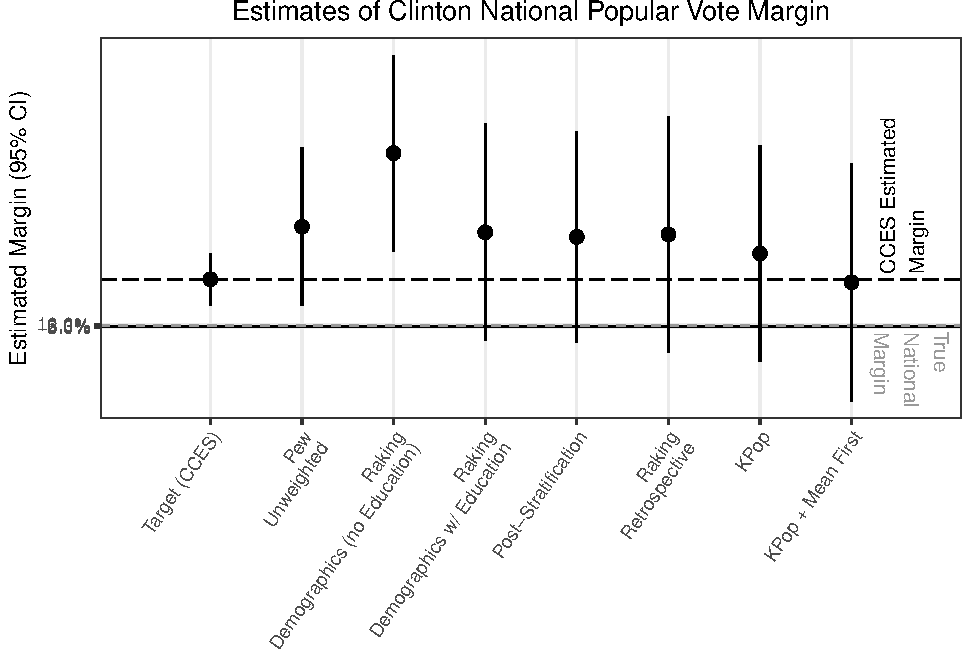
\includegraphics{application_clean_files/figure-latex/plot_results-1.pdf}

\begin{Shaded}
\begin{Highlighting}[]
\KeywordTok{ggsave}\NormalTok{(}\StringTok{"./plots/weighted_pew_results.pdf"}\NormalTok{, }\DataTypeTok{width =} \DecValTok{6}\NormalTok{, }\DataTypeTok{height =} \DecValTok{4}\NormalTok{)}
\end{Highlighting}
\end{Shaded}

\end{document}
